% Original source: Zhou, physical PDF pp. 105--109 (printed pp. 89--93).
% Figures: 4.4 and 4.5 redrawn natively with TikZ.
% Uncertainty log: none.

% ZHOU-SOURCE-PAGE: 105 PRINTED: 89

\begin{figure}[ht]
\centering
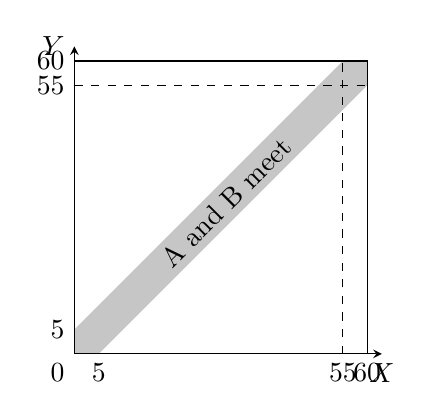
\begin{tikzpicture}[x=0.062cm,y=0.062cm,>=stealth]
  \fill[gray!45] (0,0) -- (5,0) -- (60,55) -- (60,60) -- (55,60) -- (0,5) -- cycle;
  \draw (0,0) rectangle (60,60);
  \draw[dashed] (0,55) -- (60,55);
  \draw[dashed] (55,0) -- (55,60);
  \draw[->] (0,0) -- (63,0) node[below] {$X$};
  \draw[->] (0,0) -- (0,63) node[left] {$Y$};
  \node[below left] at (0,0) {$0$};
  \node[below] at (5,0) {$5$};
  \node[below] at (55,0) {$55$};
  \node[below] at (60,0) {$60$};
  \node[left] at (0,5) {$5$};
  \node[left] at (0,55) {$55$};
  \node[left] at (0,60) {$60$};
  \node[rotate=45] at (31,31) {A and B meet};
\end{tikzpicture}
\caption{Distributions of Banker A's and Banker B's arrival times}
\label{fig:zhou-figure-4-4}
\end{figure}

\subsubsection{Probability of triangle}

\begin{problem}{Probability of triangle}
A stick is cut twice randomly (each cut point follows a uniform distribution on the stick),
what is the probability that the 3 segments can form a triangle?\footnote[22]{Hint: Let the
first cut point be $x$, the second one be $y$, use the figure to show the distribution of $x$
and $y$.}
\end{problem}
\begin{solution}
Without loss of generality, let's assume that the length of the stick is 1. Let's
also label the point of the first cut as $x$ and the second cut as $y$.

If $x<y$, then the three segments are $x$, $y-x$ and $1-y$. The conditions to form a
triangle are

\begin{center}
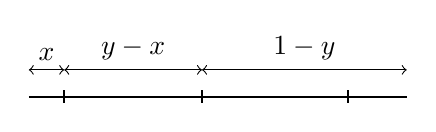
\begin{tikzpicture}[x=1cm,y=1cm]
  \draw[thick] (0,0) -- (4.8,0);
  \draw[thick] (0.45,0.08) -- (0.45,-0.08);
  \draw[thick] (2.2,0.08) -- (2.2,-0.08);
  \draw[thick] (4.05,0.08) -- (4.05,-0.08);
  \draw[<->] (0,0.34) -- (0.45,0.34) node[midway,above] {$x$};
  \draw[<->] (0.45,0.34) -- (2.2,0.34) node[midway,above] {$y-x$};
  \draw[<->] (2.2,0.34) -- (4.8,0.34) node[midway,above] {$1-y$};
\end{tikzpicture}
\end{center}

\begin{align*}
x+(y-x)&>1-y \Rightarrow y>1/2,\\
x+(1-y)&>y-x \Rightarrow y<1/2+x,\\
(y-x)+(1-y)&>x \Rightarrow x<1/2.
\end{align*}

The feasible area is shown in Figure 4.5. The case for $x<y$ is the left gray
triangle. Using symmetry, we can see that the case for $x>y$ is the right gray
triangle.

\begin{figure}[ht]
\centering
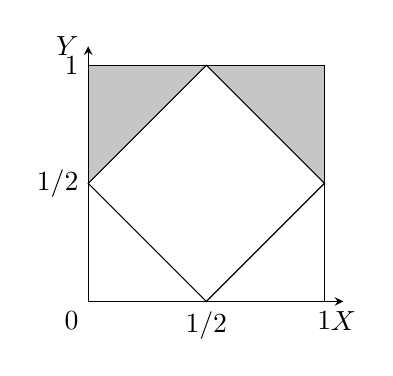
\begin{tikzpicture}[x=3.0cm,y=3.0cm,>=stealth]
  \fill[gray!45] (0,0.5) -- (0,1) -- (0.5,1) -- cycle;
  \fill[gray!45] (0.5,1) -- (1,1) -- (1,0.5) -- cycle;
  \draw (0,0) rectangle (1,1);
  \draw (0,0.5) -- (0.5,1) -- (1,0.5) -- (0.5,0) -- cycle;
  \draw[->] (0,0) -- (1.08,0) node[below] {$X$};
  \draw[->] (0,0) -- (0,1.08) node[left] {$Y$};
  \node[below left] at (0,0) {$0$};
  \node[below] at (0.5,0) {$1/2$};
  \node[below] at (1,0) {$1$};
  \node[left] at (0,0.5) {$1/2$};
  \node[left] at (0,1) {$1$};
\end{tikzpicture}
\caption{Distribution of cuts X and Y}
\label{fig:zhou-figure-4-5}
\end{figure}

% ZHOU-SOURCE-PAGE: 106 PRINTED: 90

The total shadowed area represents the region where 3 segments can form a triangle,
which is 1/4 of the square. So the probability is 1/4.
\end{solution}

\subsubsection{Property of Poisson process}

\begin{problem}{You are waiting for a bus at a bus station. The buses arrive at the station according to a Poisson process with an average arrival time of 10 minutes ($\lambda=0.1/\min$). If the buses have been running for a long time and you arrive at the bus station at a random time, what is your expected waiting time? On average, how many minutes ago did the last bus leave?}

\end{problem}
\begin{solution}
Considering the importance of jump-diffusion processes in derivative pricing and the
role of Poisson processes in studying jump processes, let's elaborate more on
exponential random variables and the Poisson process. Exponential distribution is widely
used to model the time interval between independent events that happen at a constant
average rate (arrival rate) $\lambda$:

\[
f(t)=
\begin{cases}
\lambda e^{-\lambda t}, & (t\ge 0)\\
0, & (t<0)
\end{cases}.
\]

The expected arrival time is $1/\lambda$ and the variance is $1/\lambda^2$. Using
integration, we can calculate the \(\CDF\) of an exponential distribution to be
$F(t)=P(\tau\le t)=1-e^{-\lambda t}$ and $P(\tau>t)=e^{-\lambda t}$, where $\tau$ is
the random variable for arrival time. One unique property of exponential distribution is
memorylessness: $P\{\tau>s+t\vert\tau>s\}=P(\tau>t)$.\footnote[23]{$P\{\tau>s+t\vert\tau>s\}=e^{-\lambda(s+t)}/e^{-\lambda s}=e^{-\lambda t}=P(\tau>t)$.}
That means if we have waited for $s$ time units, the extra waiting time has the same
distribution as the waiting time when we start at time 0.

When the arrivals of a series of events each independently follow an exponential
distribution with arrival rate $\lambda$, \emph{the number of arrivals between time 0 and
$t$} can be modeled as a Poisson process
$P(N(t)=x)=\dfrac{e^{-\lambda t}\lambda t^x}{x!},\quad x=0,1,\ldots$.\footnote[24]{More rigorously, $N(t)$ is defined as a right-continuous function.}
The expected number of arrivals is $\lambda t$ and the variance is also $\lambda t$.
Because of the memoryless nature of exponential distribution, the number of arrivals
between time $s$ and $t$ is also a Poisson process
\[
P(N(t-s)=x)=\frac{e^{-\lambda(t-s)}\left(\lambda(t-s)\right)^x}{x!}.
\]

Taking advantage of the memoryless property of exponential distribution, we know that
the expected waiting time is $1/\lambda=10\min$. If you look back in time, the
memoryless property still applies. So on average, the last bus arrived 10 minutes ago as
well.

% ZHOU-SOURCE-PAGE: 107 PRINTED: 91

This is another example that your intuition may misguide you. You may be wondering that
if the last bus on average arrived 10 minutes ago and the next bus on average will arrive
10 minutes later, shouldn't the average arrival time be 20 minutes instead of 10? The
explanation to the apparent discrepancy is that when you arrive at a random time, you are
more likely to arrive in a long time interval between two bus arrivals than in a short one.
For example, if one interval between two bus arrivals is 30 minutes and another is 5
minutes, you are more likely to arrive at a time during that 30-minute interval rather
than 5-minute interval. In fact, if you arrive at a random time, the expected residual
life (the time for the next bus to arrive) is $\dfrac{\E[X^2]}{2\E[X]}$ for a general
distribution.\footnote[25]{The residual life is explained in Chapter 3 of ``\textit{Discrete Stochastic Process}'' by Robert G. Gallager.}
\end{solution}

\subsubsection{Moments of normal distribution}

\begin{problem}{If $X$ follows standard normal distribution ($X\sim N(0,1)$), what is $\E[X^n]$ for $n=1,2,3$ and 4?}

\end{problem}
\begin{solution}
The first to fourth moments of the standard normal distribution are essentially the mean,
the variance, the skewness and the kurtosis. So you probably have remembered that the
answers are 0, 1, 0 (no skewness), and 3, respectively.

Standard normal distribution has \(\PDF\) $f(x)=\dfrac{1}{\sqrt{2\pi}}e^{-x^2/2}$. Using
simple symmetry we have
\[
\E[x^n]=\int_{-\infty}^{\infty}x^n\frac{1}{\sqrt{2\pi}}e^{-x^2/2}\,\dd x=0
\]
when $n$ is odd. For $n=2$, integration by parts are often used. To solve $\E[X^n]$ for
any integer $n$, an approach using \emph{moment generating functions} may be a better
choice. Moment generating functions are defined as

\[
M(t)=\E[e^{tx}]=
\begin{cases}
\displaystyle\sum_x e^{tx}p(x), & \text{if }x\text{ is discrete},\\[6pt]
\displaystyle\int_{-\infty}^{\infty}e^{tx}f(x)\,\dd x, & \text{if }x\text{ is continuous}.
\end{cases}
\]

Sequentially taking derivative of $M(t)$, we get one frequently-used property of
$M(t)$:
\[
M'(t)=\frac{\dd}{\dd t}\E[e^{tx}]=\E[Xe^{tx}]\Rightarrow M'(0)=\E[X],
\]
\[
M''(t)=\frac{\dd}{\dd t}\E[Xe^{tx}]=\E[X^2e^{tx}]\Rightarrow M''(0)=\E[X^2].
\]

% ZHOU-SOURCE-PAGE: 108 PRINTED: 92

and $M^n(0)=\E[X^n],\ \forall n\ge 1$ in general.

We can use this property to solve $\E[X^n]$ for $X\sim N(0,1)$. For standard normal
distribution
\[
\begin{aligned}
M(t)&=\E[e^{tX}]=\int_{-\infty}^{\infty}e^{tx}\frac{1}{\sqrt{2\pi}}e^{-x^2/2}\,\dd x\\
&=e^{t^2/2}\int_{-\infty}^{\infty}\frac{1}{\sqrt{2\pi}}e^{-(x-t)^2/2}\,\dd x=e^{t^2/2}.
\end{aligned}
\]

(The factor $\dfrac{1}{\sqrt{2\pi}}e^{-(x-t)^2/2}$ is the \(\PDF\) of normal distribution
$X\sim N(t,1)$, so $\int_{-\infty}^{\infty}f(x)\,\dd x=1$.)

Taking derivatives, we have
\[
M'(t)=te^{t^2/2}\Rightarrow M'(0)=0,\quad
M''(t)=e^{t^2/2}+t^2e^{t^2/2}\Rightarrow M''(0)=e^0=1,
\]
\[
\begin{aligned}
M'''(t)&=te^{t^2/2}+2te^{t^2/2}+t^3e^{t^2/2}\\
&=3te^{t^2/2}+t^3e^{t^2/2}\Rightarrow M'''(0)=0,
\end{aligned}
\]
\[
\begin{aligned}
M^{4}(t)&=3e^{t^2/2}+3t^2e^{t^2/2}+3t^2e^{t^2/2}+3t^4e^{t^2/2}\\
&\Rightarrow M^{4}(0)=3e^0=3.
\end{aligned}
\]
\end{solution}

\subsection{Expected Value, Variance \& Covariance}

Expected value, variance and covariance are indispensable in estimating returns and risks
of any investments. Naturally, they are a popular test subject in interviews as well. The
basic knowledge includes the following:

If $\E[x_i]$ is finite for all $i=1,\ldots,n$, then
$\E[X_1+\cdots+X_n]=\E[X_1]+\cdots+\E[X_n]$. The relationship holds whether the $x_i$'s
are independent of each other or not.

If $X$ and $Y$ are independent, then $\E[g(X)h(Y)]=\E[g(x)]\E[h(Y)]$.

\noindent\emph{Covariance:} $\operatorname{cov}(X,Y)=\E[(X-\E[X])(Y-\E[Y])]=\E[XY]-\E[X]\E[Y]$.

\noindent\emph{Correlation:} $\rho(X,Y)=\dfrac{\operatorname{cov}(X,Y)}{\sqrt{\operatorname{var}(X)\operatorname{var}(Y)}}$.

If $X$ and $Y$ are independent, $\operatorname{cov}(X,Y)=0$ and $\rho(X,Y)=0$.\footnote[26]{The reverse is not true. $\rho(X,Y)=0$ only means $X$ and $Y$ are uncorrelated; they may well be dependent.}

\noindent\emph{General rules of variance and covariance:}
\[
\begin{aligned}
\operatorname{cov}\left(\sum_{i=1}^{n}a_i x_i,\sum_{j=1}^{m}b_j y_j\right)
&=\sum_{i=1}^{n}\sum_{j=1}^{m}a_i b_j\operatorname{cov}(X_i,Y_j)
\end{aligned}
\]
\[
\begin{aligned}
\operatorname{var}\left(\sum_{i=1}^{n}X_i\right)
&=\sum_{i=1}^{n}\operatorname{var}(X_i)+2\sum_{i<j}\operatorname{cov}(X_i,X_j).
\end{aligned}
\]

% ZHOU-SOURCE-PAGE: 109 PRINTED: 93

\subsubsection{Conditional expectation and variance}

For discrete distribution:
$\E[g(X)\vert Y=y]=\sum_xg(x)p_{X\vert Y}(x\vert y)=\sum_xg(x)p(X=x\vert Y=y)$

For continuous distribution:
$\E[g(X)\vert Y=y]=\int_{-\infty}^{\infty}g(x)f_{X\vert Y}(x\vert y)\,\dd x$

\noindent\emph{Law of total expectation:}
\[
\E[X]=\E[\E[X\vert Y]]=
\begin{cases}
\displaystyle\sum_y \E[X\vert Y=y]p(Y=y), & \text{for discrete }Y,\\[6pt]
\displaystyle\int_{-\infty}^{\infty}\E[X\vert Y=y]f_Y(y)\,\dd y, & \text{for continuous }Y.
\end{cases}
\]

\subsubsection{Connecting noodles}

\begin{problem}{You have 100 noodles in your soup bowl. Being blindfolded, you are told to take two ends of some noodles (each end on any one noodle has the same probability of being chosen) in your bowl and connect them. You continue until there are no free ends. The number of loops formed by the noodles this way is stochastic. Calculate the expected number of circles.}

\end{problem}
\begin{solution}
Again do not be frightened by the large number 100. If you have no clue how to start,
let's begin with the simplest case where $n=1$. Surely you have only one choice (to
connect both ends of the noodle), so $\E[f(1)]=1$. How about 2 noodles? Now you have 4
ends ($2\cdot2$) and you can connect any two of them. There are
$\binom{4}{2}=\dfrac{4\cdot3}{2}=6$ combinations. Among them, 2 combinations will
connect both ends of the same noodle together and yield 1 circle and 1 noodle. The other
4 choices will yield a single noodle. So the expected number of circles is
\[
\begin{aligned}
\E[f(2)]&=\frac{2}{6}\cdot(1+\E[f(1)])+\frac{4}{6}\cdot\E[f(1)]\\
&=\frac{1}{3}+\E[f(1)]=\frac{1}{3}+1.
\end{aligned}
\]

We now move on to 3 noodles with $\binom{6}{2}=\dfrac{6\cdot5}{2}=15$ choices. Among
them, 3 choices will yield 1 circle and 2 noodles; the other 12 choices will yield 2
noodles only, so
\[
\begin{aligned}
\E[f(3)]&=\frac{3}{15}\cdot(1+\E[f(2)])+\frac{12}{15}\cdot\E[f(2)]\\
&=\frac{1}{5}+\E[f(2)]=\frac{1}{5}+\frac{1}{3}+1.
\end{aligned}
\]

See the pattern? For any $n$ noodles, we will have
$\E[f(n)]=1+1/3+1/5+\cdots+1/(2n-1)$, which can be easily proved by induction. Plug
100 in, we will have the answer.
